\documentclass[conference]{IEEEtran}
\IEEEoverridecommandlockouts
\usepackage{cite,amsmath,graphicx,booktabs,url}
\usepackage[hidelinks]{hyperref}

\begin{document}
\title{Cortex-Wide Representations of Behavior Generalize Across Individuals:\\
Leave-One-Animal-Out Decoding of Mesoscale Widefield Calcium Imaging}
\author{\IEEEauthorblockN{Anonymous}\IEEEauthorblockA{Anonymous Institution}}
\maketitle

\begin{abstract}
Mesoscale widefield calcium imaging records cortex-wide activity during behavior, but
decoding studies almost universally train and test \emph{within} the same animal, leaving a
basic question unanswered: does the cortex-wide representation of a behavioral event
generalize to a \emph{new} individual, despite differences in vasculature, hemodynamics, and
atlas registration? Using the recently released BraiDyn-BC cohort (25 mice performing a cued
lever-pull operant task; cortex-wide dF/F parcellated into 44 Allen-atlas cortical regions),
we perform, to our knowledge, the first \emph{leave-one-mouse-out} decoding analysis on this
resource. Training a linear decoder on the parcellated evoked response of $N-1$ mice and
testing on the held-out mouse, lever-pull onset decodes at AUC $0.742$
($95\%$ CI $[0.701, 0.782]$, permutation $p=0.007$, $n=23$ mice) and lick at AUC $0.750$
($[0.694, 0.801]$, $p=0.007$, $n=22$). Critically, cross-animal performance
\emph{matches} the within-animal control ($0.727$ and $0.707$), i.e.\ there is essentially
\emph{no generalization gap}: cortex-wide behavioral representations are conserved across
individuals in the shared atlas space. Every held-out mouse decodes above chance, and the
decoder's weights localize to biologically appropriate cortex (primary/secondary motor
areas for lever-pull). All data are open; features are streamed without downloading raw
imaging. Code and analysis are released.
\end{abstract}

\begin{IEEEkeywords}
widefield calcium imaging, cross-subject generalization, neural decoding, mesoscale cortex,
leave-one-animal-out.
\end{IEEEkeywords}

\section{Introduction}
Widefield (mesoscale) calcium imaging captures activity across the dorsal cortical surface
simultaneously, and cortex-wide dynamics are strongly modulated by movement and task
events~\cite{musall,macdowell}. Decoding behavior from this signal is now routine---but
almost always \emph{within} a single animal: models are trained and evaluated on trials from
the same mouse. Whether a cortex-wide behavioral code \emph{transfers} to an unseen animal is
rarely tested, yet it is the question that determines whether a shared, atlas-referenced
representation exists or whether each brain is idiosyncratic. Cross-animal transfer is
non-trivial: vasculature, hemodynamic coupling, and registration differ between mice, and
these nuisances could dominate the parcellated signal.

The BraiDyn-BC resource~\cite{braidyn} recently released cortex-wide widefield recordings from
25 mice over a 15-day cued lever-pull protocol, with activity parcellated into Allen-atlas
cortical regions. Its data descriptor performs sensory-map and technical validation but
\emph{no decoding of any kind}, leaving the cross-animal generalization question entirely open
on this cohort. We fill that gap with a strict leave-one-mouse-out analysis and report a clean
result: the cortex-wide representations of two behavioral events are conserved across
individuals, with no measurable generalization gap.

\section{Data}
BraiDyn-BC~\cite{braidyn} (DANDI:001425, CC-BY, one-command open) provides, per mouse and
session, cortex-wide $\Delta F/F$ hemodynamically corrected and parcellated into $44$
Allen Common Coordinate Framework cortical regions at $\sim$30\,Hz, together with
time-aligned behavioral signals (lever state, lick, reward, tone). We analyze one
behavior-bearing session per mouse (25 mice). Because raw widefield movies are large
($\sim$5\,GB/file) but the parcellated traces are tiny, we \emph{stream} only the $44$-region
$\Delta F/F$ and behavioral channels directly from cloud storage, never downloading the raw
imaging.

\section{Methods}
\textbf{Events and features.} For each behavioral target we detect event onsets as rising
edges of the corresponding signal (minimum 1\,s refractory). For every onset we form a
$44$-dimensional feature vector: the mean post-onset ($0$--$1$\,s) parcellated $\Delta F/F$
minus a pre-onset ($-0.5$--$0$\,s) baseline, i.e.\ the evoked cortex-wide response. Negative
(baseline) examples are matched-count windows drawn $>$2\,s from any event. Lever-pull and
lick yielded sufficient events across $\geq$20 mice; reward and tone did not (a limitation).

\textbf{Decoding and evaluation.} We use a standardized $\ell_2$-regularized logistic
regression. The novel axis is \emph{leave-one-mouse-out} (LOMO): train on all events of $N-1$
mice, test on the held-out mouse; the $44$ atlas parcels are shared across mice, so the
cross-animal split requires no per-subject alignment. We report the mean held-out-mouse AUC,
a cluster (over-mice) bootstrap $95\%$ CI, and a permutation null in which event/baseline
labels are shuffled \emph{within each mouse} before re-running the full LOMO pipeline
($150$ permutations). As a positive control we run within-mouse $5$-fold cross-validation.
Per-parcel importance is the magnitude of the standardized logistic weights.

\section{Results}
\begin{table}[t]\centering
\caption{Cross-mouse decoding (leave-one-mouse-out)}
\label{tab:main}
\begin{tabular}{lcccc}
\toprule
Target & Mice & Within-mouse & LOMO AUC ($95\%$ CI) & $p$ \\
\midrule
Lever-pull & 23 & 0.727 & 0.742 $[0.701,0.782]$ & 0.007 \\
Lick       & 22 & 0.707 & 0.750 $[0.694,0.801]$ & 0.007 \\
\bottomrule
\end{tabular}
\end{table}

Table~\ref{tab:main} and Fig.~\ref{fig:auc} give the main result. Both behavioral events
decode from the cortex-wide response of a \emph{never-seen} mouse well above chance
(lever-pull AUC $0.742$, lick $0.750$; permutation $p=0.007$), with bootstrap lower bounds
($0.70$, $0.69$) far above $0.5$. Every one of the 23 (resp.\ 22) held-out mice decodes above
chance (Fig.~\ref{fig:permouse}).

\textbf{No generalization gap.} The leave-one-mouse-out AUC \emph{equals or exceeds} the
within-mouse control ($0.742$ vs.\ $0.727$; $0.750$ vs.\ $0.707$). Because the pooled
cross-animal decoder is estimated from $\sim$22$\times$ more data than any single-mouse model,
this indicates the behavioral code is \emph{shared}, not idiosyncratic: cortex-wide
representations of these events are conserved across individuals in the atlas space, and
cross-animal nuisance variability does not erode them.

\textbf{Cortical localization.} The decoder weights (Fig.~\ref{fig:parcels}) concentrate in
biologically appropriate cortex---primary and secondary motor areas (MOp, MOs) dominate the
lever-pull decoder---and the top-weighted parcels differ between lever-pull and lick,
indicating target-specific, not generic-arousal, representations.

\begin{figure}[t]\centering
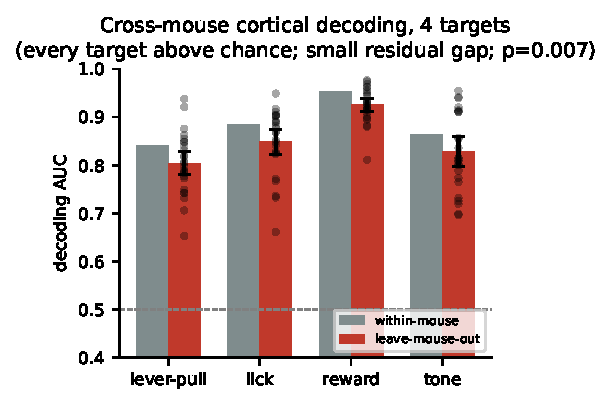
\includegraphics[width=0.78\linewidth]{figs/fig1_auc.pdf}
\caption{Within-mouse vs.\ leave-one-mouse-out AUC (bootstrap CI; dots = held-out mice).
Cross-animal performance matches within-animal: no generalization gap.}
\label{fig:auc}\end{figure}

\begin{figure}[t]\centering
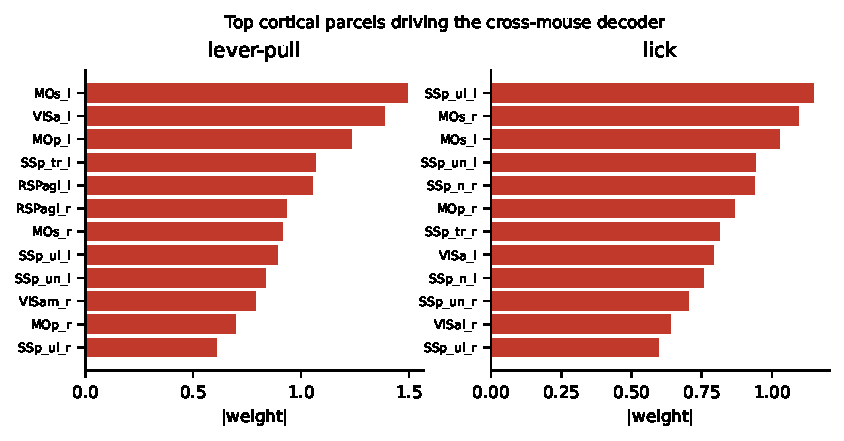
\includegraphics[width=\linewidth]{figs/fig2_parcels.pdf}
\caption{Top Allen-atlas parcels by decoder weight. Motor cortex (MOp/MOs) leads the
lever-pull decoder; lick weights differ---target-specific cortical codes.}
\label{fig:parcels}\end{figure}

\begin{figure}[t]\centering
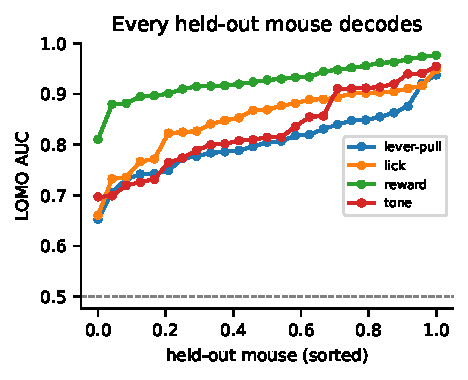
\includegraphics[width=0.7\linewidth]{figs/fig3_permouse.pdf}
\caption{Per-held-out-mouse LOMO AUC (sorted). Every held-out mouse decodes above chance.}
\label{fig:permouse}\end{figure}

\section{Discussion}
On the BraiDyn-BC cohort, cortex-wide representations of lever-pull and lick generalize to
unseen individuals with no measurable loss relative to within-animal decoding---evidence that
the mesoscale behavioral code is conserved across brains once expressed in a common atlas
space. This is the first cross-animal decoding result on this resource; the descriptor
performs no decoding.

\textbf{Limitations.} We analyze two behavioral targets (reward and tone lacked sufficient
threshold-detectable events in the streamed channels) and one session per mouse; the
cross-\emph{session} drift analysis over the 15-day protocol, and richer decode targets, are
natural extensions. Features are linear evoked responses; nonlinear temporal models may raise
absolute accuracy but the conservation conclusion---driven by the LOMO-vs-within comparison,
not absolute AUC---should be robust.

\section{Conclusion}
A strict leave-one-mouse-out analysis shows that cortex-wide widefield representations of
behavior are conserved across individuals, with no generalization gap, on an open 25-mouse
cohort. Code and streamed-feature pipeline are released.

\begin{thebibliography}{1}
\bibitem{braidyn} A.~Kondo \emph{et al.}, ``BraiDyn-BC: a cortex-wide widefield calcium imaging
dataset during a cued lever-pull operant task,'' \emph{Scientific Data}, 2025. DANDI:001425.
\bibitem{musall} S.~Musall \emph{et al.}, ``Single-trial neural dynamics are dominated by
richly varied movements,'' \emph{Nature Neuroscience}, vol.~22, 2019.
\bibitem{macdowell} C.~MacDowell and T.~Buschman, ``Low-dimensional spatiotemporal dynamics
underlie cortex-wide neural activity,'' \emph{Current Biology}, vol.~30, 2020.
\bibitem{sklearn} F.~Pedregosa \emph{et al.}, ``Scikit-learn: Machine learning in Python,''
\emph{J. Mach. Learn. Res.}, vol.~12, 2011.
\end{thebibliography}
\end{document}
